\documentclass[11pt]{beamer}
\usetheme[progressbar=frametitle]{metropolis}
\usepackage[utf8]{inputenc}
\usepackage[spanish]{babel}
\usepackage{fancyvrb}
\definecolor{new_green}{HTML}{347F1F}


\author{Lic. Agustina Pesce \\ Lic. Santiago Soler}
\title[Taller de {\LaTeX}]{Taller Introductorio a {\LaTeX}: \\ Cómo producir documentos de Calidad}
\subtitle{Segundo Encuentro: Artículo Científico}
%\setbeamercovered{transparent} 
%\setbeamertemplate{navigation symbols}{} 
%\logo{} 
%\institute{} 
\date{}
%\subject{} 

\begin{document}
\maketitle

\section{El Articulo Científico}

\begin{frame}{Estructura Básica de un Artículo Científico}
\begin{itemize}[<+- | alert@+>] % Con esto hacemos que aparezcan los items de a uno
  \item Titulo
  \item Autores
  \item Abstract
  \item Cuerpo principal (secciones y subsecciones)
\end{itemize}
\end{frame}


\section{¿Cómo se hace en \LaTeX{}?}

\begin{frame}{Article Class}
\begin{itemize}[<+- | alert@+>] % Con esto hacemos que aparezcan los items de a uno
  \item Defino en el preámbulo el tipo de documento que voy a escribir por medio del comando \textbackslash documentclass \{article\}
  \item Creo el titulo
  \item Escribo los autores
  \item Inicio el entorno llamado Abstract
  \item Escribo el cuerpo principal del texto (secciones y subsecciones)
\end{itemize}
\end{frame}

\begin{frame}[fragile]{Article Class}
\textbf{Ejemplos de un articulo en \LaTeX{}}
\begin{columns}
\column{0.5\textwidth}
{\color{new_green}
\begin{Verbatim}[fontsize=\scriptsize]
\documentclass[a4paper,12pt]{article}
\usepackage[utf8]{inputenc}

%opening
\title{Hola Mundo}
\author{Anomimo}

\begin{document}
\maketitle

\begin{abstract}
Resumen del mundo.
\end{abstract}

\section{Según Colon}
El mundo era plano.
\end{document}
\end{Verbatim}
}
\hfill
\column{0.4\textwidth}
{\scriptsize
Declaro el tipo de documento, papel y tamaño de letra. 
Defino la codificación del documento. \\
\vspace{2.5em}
Defino el titulo. \\
Defino el autor. \\
\vspace{2.5em}
Creo el titulo y el autor \\
\vspace{2.5em}
Creo el Abstract \\
\vspace{2em}
Creo una sección
\vspace{4.5em}
}
\end{columns}
\end{frame}

\begin{frame}{Article Class}
Después de compilar:
\vspace{-1em}
\begin{figure}[b]
  \centering
  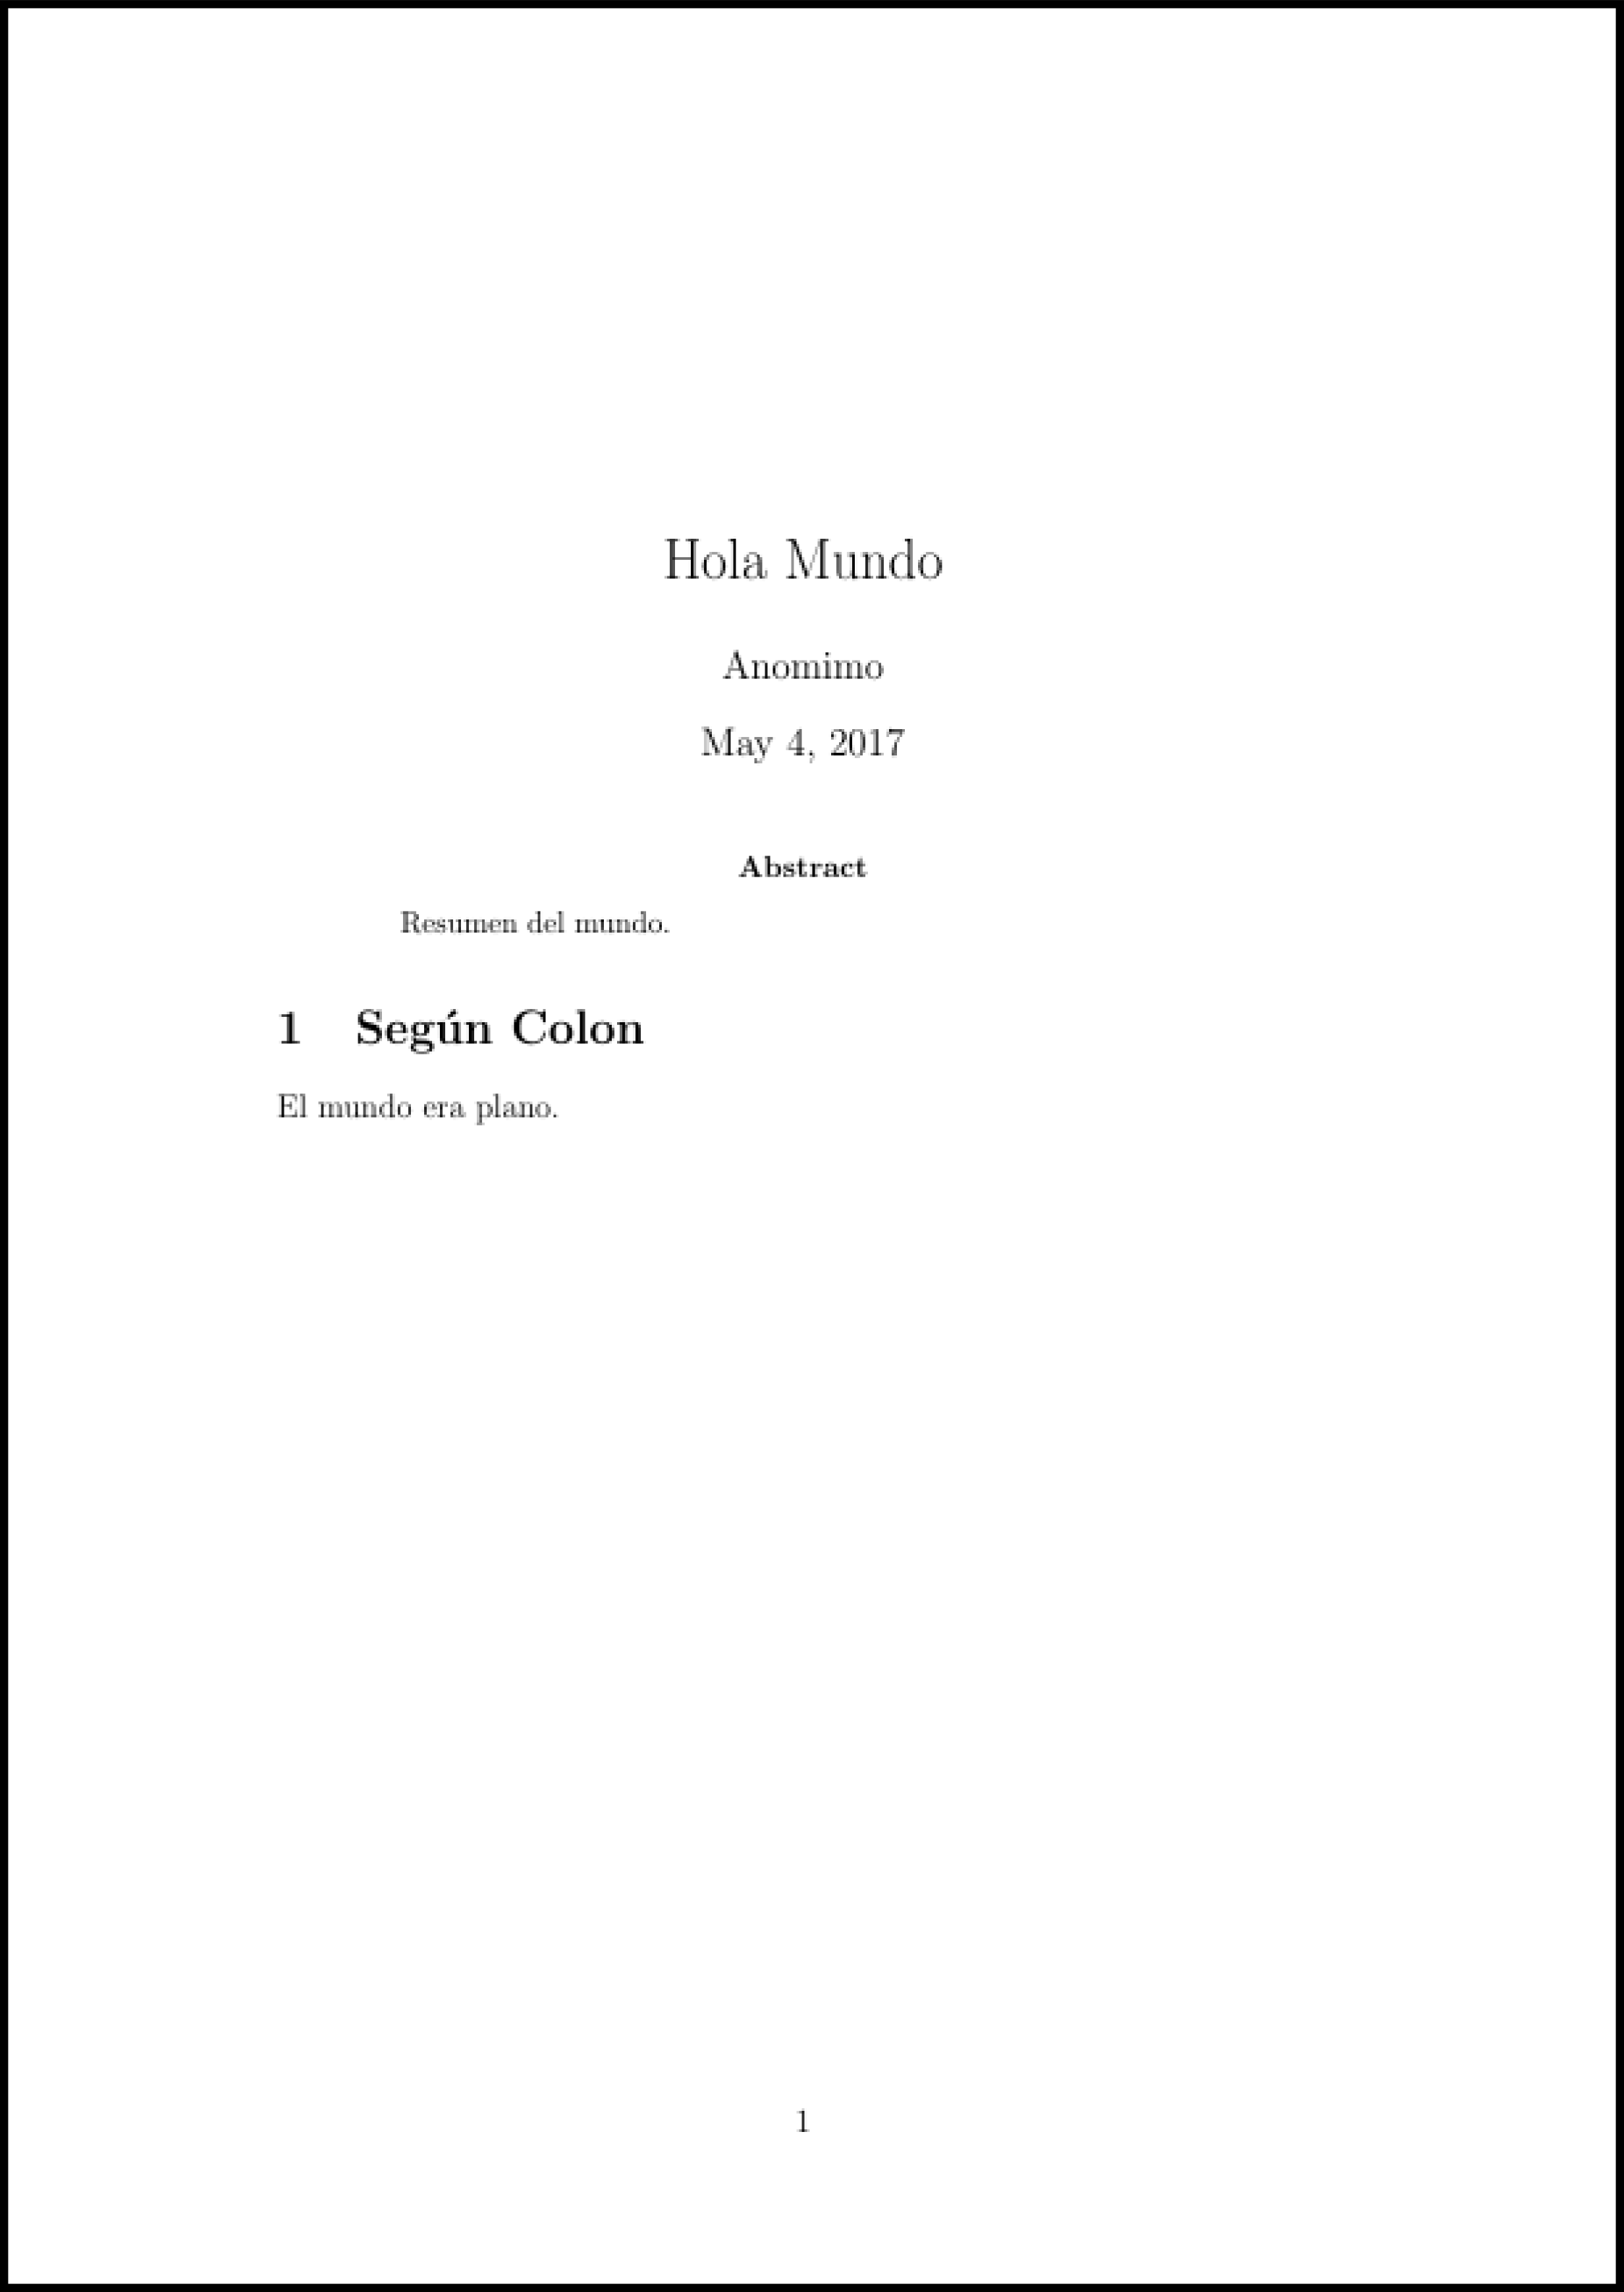
\includegraphics[width=0.45\textwidth]{figs/ej1.png}
\end{figure}
\end{frame}


\end{document}

